\section{Infrastruktur / Spannungsreferenz eines SoC}

\begin{center}
    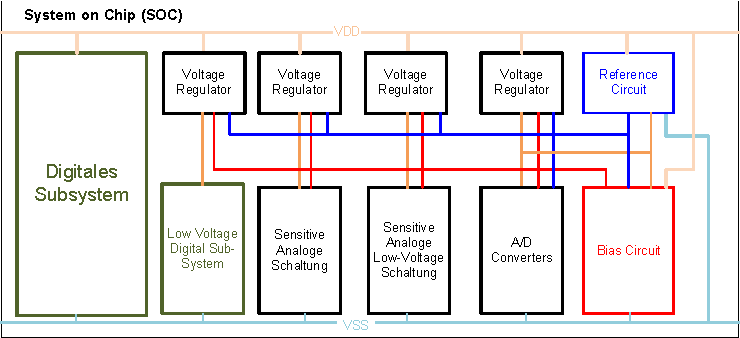
\includegraphics[width=0.8\columnwidth, align=t]{images/13_SoC.pdf}
\end{center}
\vspace{-0.2cm}


\subsection{Spannungsversorgung}
Ein wichtiger Teil der 'Infrastruktur' auf einem SoC ist die Spannungsversorgung. 
Die benötigte Leistung kann wie folgt abgeschätzt werden.
\[
    P_\mathrm{dynamisch} = f(C, f, N, U^2) \qquad \qquad
    P_\mathrm{statisch} = I_\mathrm{leakage} \cdot U^2
\]

Besonders kritisch ist das Rauschen, welches von digitalen Schaltungsblöcken erzeugt wird und für analoge Baublöcke weggefiltert werden muss.


\subsection{Arbeitspunkteinstellung mittels Bias Circuit}
Zur Arbeitspunkteinstellung gibt es verschiedene Strategien.
Diese können für einen der unten aufgeführten Punkte ausgelegt werden.

\smallskip

\begin{minipage}[t]{0.42\columnwidth}
    \begin{itemize}
        \item Konstante Spannungsamplitude
        \item Konstante Ströme
    \end{itemize}
\end{minipage}
\hfill
\begin{minipage}[t]{0.55\columnwidth}
    \begin{itemize}
        \item Konstante Verstärkung und Transkonduktanz
    \end{itemize}
\end{minipage}

\smallskip

Der erforderliche Bias-Strom wird von einer Generator-Schaltung generiert und anschliessend an die 'Verbraucher' verteilt. 


\subsubsection{Verteilungsarten}
\paragraph{Voltage Mode (nicht empfehlenswert)}

\begin{minipage}[t]{0.4\columnwidth}
    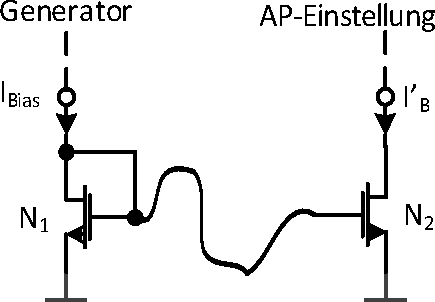
\includegraphics[width=\columnwidth, align=t]{images/13_voltage_mode.pdf}
\end{minipage}
\hfill
\begin{minipage}[t]{0.58\columnwidth}
    \raggedright
    Die Bias-Quelle besteht aus der Diode des Stromspiegels.
    Die Diodenspannung wird an alle Stromquellen-Transistoren geführt.

    \smallskip

    \begin{itemize}
        \item[+] Minimale Hardware
        \item[-] Schlechtes Matching zwischen Generator und 'Verbraucher' (aufgrund von Technologie und Temperaturvariationen)
        \item[-] \textbf{Störungen} auf der Verbindungsleitung
    \end{itemize}
\end{minipage}



\paragraph{Current Mode (bevorzugte Methode)}

\begin{minipage}[t]{0.45\columnwidth}
    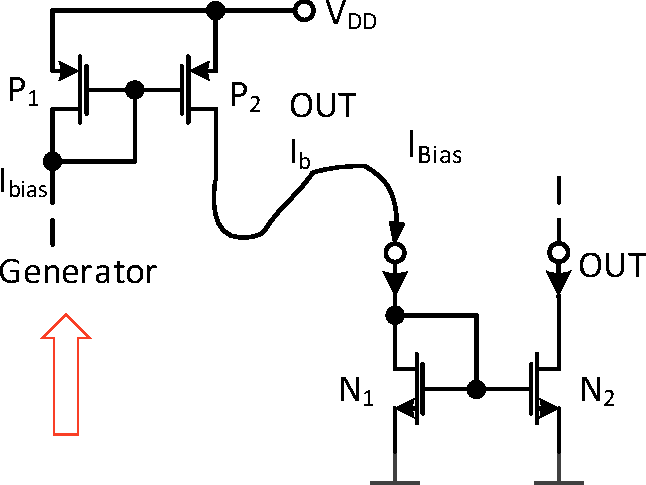
\includegraphics[width=\columnwidth, align=t]{images/13_current_mode.pdf}
\end{minipage}
\hfill
\begin{minipage}[t]{0.53\columnwidth}
    Jeder 'Verbraucher' hat am Eingang einen eigenen Stromspiegel, welcher den Bias-Strom 'reproduziert'.

    \smallskip

    \begin{itemize}
        \item[+] Gutes Matching (Stromspiegeltransistoren am gleichen Ort)
        \item[+] \textbf{Weniger störanfällig} wegen niederohmigen Signalen
        \item[-] Mehr Hardware
        \item[-] Höherer Stromverbrauch
    \end{itemize}
\end{minipage}



\subsection{Referenzschaltungen}
Spannungsregler sowie Arbeitspunkteinstellung und verschiedene Blöcke benötigen eine \textbf{absolute Referenz}.
Absolute Referenzen jedoch schwierig zu realiseren.
Eine relative Genauigkeiten bis ca. 0.1\% ist ohne trimmen möglich, während absolute Referenzwerte Losabweichungen von bis zu 40\% aufweisen.

\smallskip

Entsprechend müssen \textbf{absolute Referenzen trimmbar realisiert werden} können. \\
Als Richtwert für die Qualität einer Referenz wird die \textbf{Sensitivität} $\bm{S}$ des Referenzwerts auf die Änderung einer externen Grösse.

\subsubsection{Spannungsteiler}

Ein Spannungsteiler ist \textbf{als Referenz unbrauchbar}, da die Sensitivität $S$ zu gross ist.

\smallskip

\begin{tabular}{l l}
    \textbf{Temperatur}             & $S$ klein bei Verwendung von identischen Widerständen             \\
    \textbf{Versorgungsspannung}    & $S=1$, d.h. Schwankung wirkt sich direkt auf $V_{\rm ref}$ aus    \\
    \textbf{Prozessvariation}       & $S$ klein bei Verwendung von identischen Widerständen
\end{tabular}



\subsubsection{Bootstrap-Referenz}

Die Bootstrap-Referenz benötigt eine Start-Up Schaltung (nicht gezeichnet), da $I_D = \qty{0}{\ampere}$ auch ein stabiler AP wäre. 

\begin{minipage}[t]{0.38\columnwidth}
    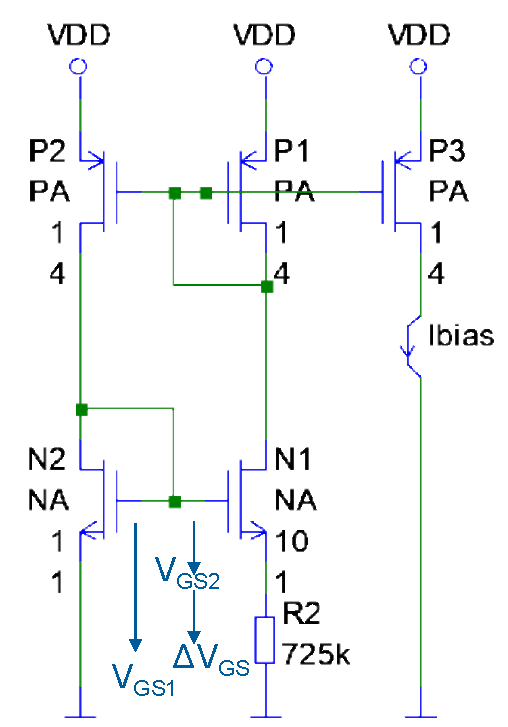
\includegraphics[width=\columnwidth, align=t]{images/13_bootstrap_referenz.pdf}
\end{minipage}
\hfill
\begin{minipage}[t]{0.58\columnwidth}
    \begin{outline}
        \1 N1 und N2 befinden sich in \textbf{weak inversion}
        \1 $R_2$: Externer Präzisionswiderstand
    \end{outline}

    \smallskip

    \[
        I_D = I_M' \frac{W}{L} e^{\frac{V_{\rm GS}-V_M}{n_m V_\mathrm{temp}}}
    \]
    \[
        V_{\rm GS} - V_M = n_m V_\mathrm{temp} \ln{\frac{I_D}{I_M' \frac{W}{L}}}
    \]
    \[
        \Delta V_{\rm GS} = V_{\rm GS1} - V_{\rm GS2} = n_m V_\mathrm{temp} \ln\left(\frac{I_{D1}}{I_{D2}} \frac{(W/L)_2}{(W/L)_1}\right)
    \]
    \[
        I_\mathrm{bias} = \frac{\Delta V_{GS}}{R_2}
    \]

    \begin{itemize}
        \item[+] Unabhängig von Versorgungsspannung ($S=0$)
        \item[-] Proportional zur Temperatur 
    \end{itemize}
\end{minipage}


\subsubsection{Bandgap-Referenz}

\begin{minipage}[c]{0.51\columnwidth}
    \paragraph{Grundprinzip}
    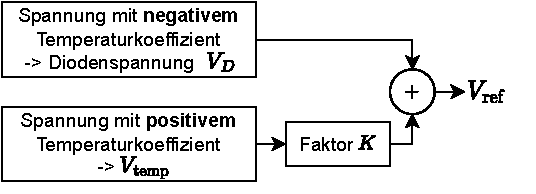
\includegraphics[width=\columnwidth, align=t]{images/13_bandgap_konzept.pdf}
\end{minipage}
\hfill
\begin{minipage}[c]{0.48\columnwidth}

    \[
        V_{\rm ref} = V_{\rm TC-} + K \cdot V_{\rm TC+} = V_D + K \cdot V_{\rm temp}
    \] 

    \textrightarrow\ Summe der Temp.-Koeffizienten muss Null sein, damit $V_{\rm ref}$ temp-unabhängig ist:
    \vspace{-0.2cm}
    \[
        \text{TC}_{\rm ref} = \text{TC}_{\rm Diode} + K \cdot  \text{TC}_{V \rm temp} \overset{!}{=} 0
    \] 
\end{minipage}

\smallskip

\[
    \text{Diode:} \qquad \text{TC}_{\rm Diode} = \qty{-2}{\milli\volt\per\kelvin} = \frac{\diff V_D}{\diff T} \approx \frac{V_D-V_{\rm BG}}{T}
\]

\[
    V_{\rm temp}: \qquad \text{TC}_{V \rm temp} = \frac{\diff V_\mathrm{temp}}{\diff T} = \frac{k}{e} \approx \qty{86.24e{-6}}{\volt\per\kelvin} 
\]

\[
    \text{Faktor:} \qquad K = -\frac{\text{TC}_{\rm Diode}}{\text{TC}_{V \mathrm{temp}}} = - \frac{\qty{-2}{\milli\volt\per\kelvin}}{\qty{86.24e{-6}}{\volt\per\kelvin}} = 23.2
\]


\paragraph{Realisierung}

\begin{minipage}[t]{0.4\columnwidth}
    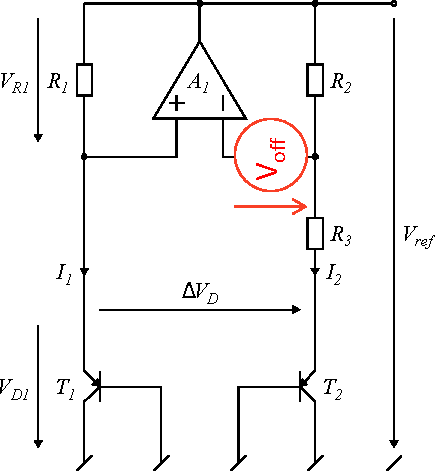
\includegraphics[width=\columnwidth, align=t]{images/13_bandgap_referenz.pdf}
\end{minipage}
\hfill
\begin{minipage}[t]{0.58\columnwidth}
    Die Bandgap-Referenz wird durch Bipolartransistoren realisiert.
    Die Emitter-Basis-Diode liefert dabei die Diodenspannung $V_D = V_{\rm EB}$.

    \smallskip

    \begin{itemize}
        \item[+] Unabhängig von Versorgungsspannung
        \item[+] \qty{10}{ppm\per\kelvin} bei (\qty{0}{\degreeCelsius}-\qty{70}{\degreeCelsius})
        \item[-] Die Spannung $V_\mathrm{ref}$ sowie der Temperaturkoeffizient hängt stark vom Offset des OpAmps ab\\
            \textrightarrow\ Trimmen
    \end{itemize}

    \smallskip

    \textbf{Hinweis:} Auch hier ist eine Startup-Schaltung nötig.
\end{minipage}

\smallskip

Die Verstärkung $K$ wird gemäss Theorie folgendermassen gefunden:
 \[
    V_{\rm ref} = V_D + K \cdot V_{\rm temp} = V_{\rm D1} + I_2 \cdot R_2 = V_{\rm D1} + \frac{V_{\rm R3}}{R_3} \cdot R_2
\] 
\[
    V_{\rm R3} = \Delta V_D = \Delta V_{\rm EB} = V_{\rm EB1} - V_{\rm EB2} = V_{\rm temp} \cdot \ln \left( \frac{I_1}{I_2} \cdot \frac{A_2}{A_1} \right)
\] 
\[
    V_{\rm ref} = V_{\rm EB1} + \frac{V_{\rm R3}}{R_3} \cdot R_2 = V_{\rm EB1} + V_{\rm temp} \cdot \frac{R_2}{R_3} \cdot \ln \left( \frac{I_1}{I_2} \cdot \frac{A_2}{A_1} \right)
\] 
\[
    K = \frac{R_2}{R_3} \cdot \ln \left( \frac{I_1}{I_2} \cdot \frac{A_2}{A_1} \right)
\] 


Unter Berücksichtigung der Offset-Spannung des OpAmps ergibt sich die Referenzspannung als:
 \[
    V_{\rm ref} = V_{\rm EB1} + V_{\rm temp} \cdot \frac{R_2}{R_3} \cdot \ln \left[  \frac{I_1}{I_2} \cdot \frac{A_2}{A_1} \cdot \left( 1 - \frac{V_{\rm off}}{R_2 I_2} \right) \right] - \left(1 + \frac{R_2}{R_3} \right) \cdot V_{\rm off}
\] 

